\documentclass[twoside]{book}

% Packages required by doxygen
\usepackage{fixltx2e}
\usepackage{calc}
\usepackage{doxygen}
\usepackage[export]{adjustbox} % also loads graphicx
\usepackage{graphicx}
\usepackage[utf8]{inputenc}
\usepackage{makeidx}
\usepackage{multicol}
\usepackage{multirow}
\PassOptionsToPackage{warn}{textcomp}
\usepackage{textcomp}
\usepackage[nointegrals]{wasysym}
\usepackage[table]{xcolor}

% Font selection
\usepackage[T1]{fontenc}
\usepackage[scaled=.90]{helvet}
\usepackage{courier}
\usepackage{amssymb}
\usepackage{sectsty}
\renewcommand{\familydefault}{\sfdefault}
\allsectionsfont{%
  \fontseries{bc}\selectfont%
  \color{darkgray}%
}
\renewcommand{\DoxyLabelFont}{%
  \fontseries{bc}\selectfont%
  \color{darkgray}%
}
\newcommand{\+}{\discretionary{\mbox{\scriptsize$\hookleftarrow$}}{}{}}

% Page & text layout
\usepackage{geometry}
\geometry{%
  a4paper,%
  top=2.5cm,%
  bottom=2.5cm,%
  left=2.5cm,%
  right=2.5cm%
}
\tolerance=750
\hfuzz=15pt
\hbadness=750
\setlength{\emergencystretch}{15pt}
\setlength{\parindent}{0cm}
\setlength{\parskip}{3ex plus 2ex minus 2ex}
\makeatletter
\renewcommand{\paragraph}{%
  \@startsection{paragraph}{4}{0ex}{-1.0ex}{1.0ex}{%
    \normalfont\normalsize\bfseries\SS@parafont%
  }%
}
\renewcommand{\subparagraph}{%
  \@startsection{subparagraph}{5}{0ex}{-1.0ex}{1.0ex}{%
    \normalfont\normalsize\bfseries\SS@subparafont%
  }%
}
\makeatother

% Headers & footers
\usepackage{fancyhdr}
\pagestyle{fancyplain}
\fancyhead[LE]{\fancyplain{}{\bfseries\thepage}}
\fancyhead[CE]{\fancyplain{}{}}
\fancyhead[RE]{\fancyplain{}{\bfseries\leftmark}}
\fancyhead[LO]{\fancyplain{}{\bfseries\rightmark}}
\fancyhead[CO]{\fancyplain{}{}}
\fancyhead[RO]{\fancyplain{}{\bfseries\thepage}}
\fancyfoot[LE]{\fancyplain{}{}}
\fancyfoot[CE]{\fancyplain{}{}}
\fancyfoot[RE]{\fancyplain{}{\bfseries\scriptsize Generated by Doxygen }}
\fancyfoot[LO]{\fancyplain{}{\bfseries\scriptsize Generated by Doxygen }}
\fancyfoot[CO]{\fancyplain{}{}}
\fancyfoot[RO]{\fancyplain{}{}}
\renewcommand{\footrulewidth}{0.4pt}
\renewcommand{\chaptermark}[1]{%
  \markboth{#1}{}%
}
\renewcommand{\sectionmark}[1]{%
  \markright{\thesection\ #1}%
}

% Indices & bibliography
\usepackage{natbib}
\usepackage[titles]{tocloft}
\setcounter{tocdepth}{3}
\setcounter{secnumdepth}{5}
\makeindex

% Hyperlinks (required, but should be loaded last)
\usepackage{ifpdf}
\ifpdf
  \usepackage[pdftex,pagebackref=true]{hyperref}
\else
  \usepackage[ps2pdf,pagebackref=true]{hyperref}
\fi
\hypersetup{%
  colorlinks=true,%
  linkcolor=blue,%
  citecolor=blue,%
  unicode%
}

% Custom commands
\newcommand{\clearemptydoublepage}{%
  \newpage{\pagestyle{empty}\cleardoublepage}%
}

\usepackage{caption}
\captionsetup{labelsep=space,justification=centering,font={bf},singlelinecheck=off,skip=4pt,position=top}

%===== C O N T E N T S =====

\begin{document}

% Titlepage & ToC
\hypersetup{pageanchor=false,
             bookmarksnumbered=true,
             pdfencoding=unicode
            }
\pagenumbering{alph}
\begin{titlepage}
\vspace*{7cm}
\begin{center}%
{\Large Vetor \\[1ex]\large 0.\+0.\+1 }\\
\vspace*{1cm}
{\large Generated by Doxygen 1.8.13}\\
\end{center}
\end{titlepage}
\clearemptydoublepage
\pagenumbering{roman}
\tableofcontents
\clearemptydoublepage
\pagenumbering{arabic}
\hypersetup{pageanchor=true}

%--- Begin generated contents ---
\chapter{Class Index}
\section{Class List}
Here are the classes, structs, unions and interfaces with brief descriptions\+:\begin{DoxyCompactList}
\item\contentsline{section}{\hyperlink{class_vetor}{Vetor} \\*A classe \hyperlink{class_vetor}{Vetor} lida com vetores bidimensionais }{\pageref{class_vetor}}{}
\end{DoxyCompactList}

\chapter{File Index}
\section{File List}
Here is a list of all files with brief descriptions\+:\begin{DoxyCompactList}
\item\contentsline{section}{\hyperlink{main_8cpp}{main.\+cpp} }{\pageref{main_8cpp}}{}
\item\contentsline{section}{\hyperlink{vetor_8cpp}{vetor.\+cpp} }{\pageref{vetor_8cpp}}{}
\item\contentsline{section}{\hyperlink{vetor_8h}{vetor.\+h} }{\pageref{vetor_8h}}{}
\end{DoxyCompactList}

\chapter{Class Documentation}
\hypertarget{class_vetor}{}\section{Vetor Class Reference}
\label{class_vetor}\index{Vetor@{Vetor}}


A classe \hyperlink{class_vetor}{Vetor} lida com vetores bidimensionais.  




{\ttfamily \#include $<$vetor.\+h$>$}

\subsection*{Public Member Functions}
\begin{DoxyCompactItemize}
\item 
\hyperlink{class_vetor_a475c943b2c1db890afc6c7958edea303}{Vetor} (float \+\_\+x=0, float \+\_\+y=0)
\begin{DoxyCompactList}\small\item\em \hyperlink{class_vetor}{Vetor} eh o construtor da classe. \end{DoxyCompactList}\item 
\hyperlink{class_vetor_a63ba9d34a0a98b151f3d85c2b4f54278}{Vetor} (\hyperlink{class_vetor}{Vetor} \&v)
\item 
\hyperlink{class_vetor_a7396a0492de44676a977c593d36e061c}{$\sim$\+Vetor} ()
\item 
void \hyperlink{class_vetor_a45e972d26987116ae8c89fefb09f5737}{setX} (float \+\_\+x)
\item 
float \hyperlink{class_vetor_a0b43068a518a1b9e42a2031aa6c41f0d}{getX} (void)
\item 
void \hyperlink{class_vetor_a25c01341d46beebd3f4bf054d576772e}{setY} (float \+\_\+y)
\item 
float \hyperlink{class_vetor_aec52a87477cfeb998a1668abae852373}{getY} (void)
\item 
float \hyperlink{class_vetor_a26e8c7db35c90a9313cfcb780a1ab324}{norma} ()
\item 
float \hyperlink{class_vetor_ab9cd8d5a657eee8a0e0b4cda209b931d}{teta} ()
\item 
void \hyperlink{class_vetor_a253a700dc67db860e2ae8247f114990e}{print} (void)
\item 
void \hyperlink{class_vetor_a77932d982688b592b82c189e08ad94d1}{negativo} (void)
\item 
void \hyperlink{class_vetor_a1374cc636a82d6f038219fd29891133e}{negativo} (int mode)
\item 
\hyperlink{class_vetor}{Vetor} \hyperlink{class_vetor_a32c6e9bcc96a7d54b3b2fe1d3c0d84c1}{soma} (\hyperlink{class_vetor}{Vetor} v)
\item 
\hyperlink{class_vetor}{Vetor} \hyperlink{class_vetor_aab0e480dfe6eaa15a5f58b1f44efcdb5}{subtracao} (\hyperlink{class_vetor}{Vetor} v)
\item 
\hyperlink{class_vetor}{Vetor} \hyperlink{class_vetor_a3d3822b8ee1525b724b15db40d798ec7}{multiplicacao} (float a)
\item 
\hyperlink{class_vetor}{Vetor} \hyperlink{class_vetor_a6c98e035c2164efb70c1e4158ff3a30e}{operator+} (\hyperlink{class_vetor}{Vetor} v)
\item 
\hyperlink{class_vetor}{Vetor} \hyperlink{class_vetor_a7e778b3bcf5c142316efc40922f325ff}{operator-\/} (\hyperlink{class_vetor}{Vetor} v)
\item 
\hyperlink{class_vetor}{Vetor} \hyperlink{class_vetor_a02b8c1a9f2d9d9701e553e4d31a3b841}{operator$\ast$} (float a)
\item 
float \hyperlink{class_vetor_ae632976a4d2f4e0479999f20a085843e}{operator$\ast$} (\hyperlink{class_vetor}{Vetor} v)
\item 
\hyperlink{class_vetor}{Vetor} \hyperlink{class_vetor_a57108f1730fe7b165e481fcc67e41d74}{operator++} ()
\item 
\hyperlink{class_vetor}{Vetor} \hyperlink{class_vetor_ac542166c6ef82d5d0f10e8a70242ed81}{operator++} (int)
\end{DoxyCompactItemize}
\subsection*{Friends}
\begin{DoxyCompactItemize}
\item 
\hyperlink{class_vetor}{Vetor} \hyperlink{class_vetor_a94de46a0867046d0a49eb7e47b6d8e36}{operator$\ast$} (float a, \hyperlink{class_vetor}{Vetor} v)
\end{DoxyCompactItemize}


\subsection{Detailed Description}
A classe \hyperlink{class_vetor}{Vetor} lida com vetores bidimensionais. 

Ela permite realizar operações entre eles. 

\subsection{Constructor \& Destructor Documentation}
\mbox{\Hypertarget{class_vetor_a475c943b2c1db890afc6c7958edea303}\label{class_vetor_a475c943b2c1db890afc6c7958edea303}} 
\index{Vetor@{Vetor}!Vetor@{Vetor}}
\index{Vetor@{Vetor}!Vetor@{Vetor}}
\subsubsection{\texorpdfstring{Vetor()}{Vetor()}\hspace{0.1cm}{\footnotesize\ttfamily [1/2]}}
{\footnotesize\ttfamily Vetor\+::\+Vetor (\begin{DoxyParamCaption}\item[{float}]{\+\_\+x = {\ttfamily 0},  }\item[{float}]{\+\_\+y = {\ttfamily 0} }\end{DoxyParamCaption})}



\hyperlink{class_vetor}{Vetor} eh o construtor da classe. 


\begin{DoxyParams}{Parameters}
{\em \+\_\+x} & valor inicial da variavel x \\
\hline
{\em \+\_\+y} & valor inicial da variavel y \\
\hline
\end{DoxyParams}
\mbox{\Hypertarget{class_vetor_a63ba9d34a0a98b151f3d85c2b4f54278}\label{class_vetor_a63ba9d34a0a98b151f3d85c2b4f54278}} 
\index{Vetor@{Vetor}!Vetor@{Vetor}}
\index{Vetor@{Vetor}!Vetor@{Vetor}}
\subsubsection{\texorpdfstring{Vetor()}{Vetor()}\hspace{0.1cm}{\footnotesize\ttfamily [2/2]}}
{\footnotesize\ttfamily Vetor\+::\+Vetor (\begin{DoxyParamCaption}\item[{\hyperlink{class_vetor}{Vetor} \&}]{v }\end{DoxyParamCaption})}

\mbox{\Hypertarget{class_vetor_a7396a0492de44676a977c593d36e061c}\label{class_vetor_a7396a0492de44676a977c593d36e061c}} 
\index{Vetor@{Vetor}!````~Vetor@{$\sim$\+Vetor}}
\index{````~Vetor@{$\sim$\+Vetor}!Vetor@{Vetor}}
\subsubsection{\texorpdfstring{$\sim$\+Vetor()}{~Vetor()}}
{\footnotesize\ttfamily Vetor\+::$\sim$\+Vetor (\begin{DoxyParamCaption}{ }\end{DoxyParamCaption})}



\subsection{Member Function Documentation}
\mbox{\Hypertarget{class_vetor_a0b43068a518a1b9e42a2031aa6c41f0d}\label{class_vetor_a0b43068a518a1b9e42a2031aa6c41f0d}} 
\index{Vetor@{Vetor}!getX@{getX}}
\index{getX@{getX}!Vetor@{Vetor}}
\subsubsection{\texorpdfstring{get\+X()}{getX()}}
{\footnotesize\ttfamily float Vetor\+::getX (\begin{DoxyParamCaption}\item[{void}]{ }\end{DoxyParamCaption})}

\mbox{\Hypertarget{class_vetor_aec52a87477cfeb998a1668abae852373}\label{class_vetor_aec52a87477cfeb998a1668abae852373}} 
\index{Vetor@{Vetor}!getY@{getY}}
\index{getY@{getY}!Vetor@{Vetor}}
\subsubsection{\texorpdfstring{get\+Y()}{getY()}}
{\footnotesize\ttfamily float Vetor\+::getY (\begin{DoxyParamCaption}\item[{void}]{ }\end{DoxyParamCaption})}

\mbox{\Hypertarget{class_vetor_a3d3822b8ee1525b724b15db40d798ec7}\label{class_vetor_a3d3822b8ee1525b724b15db40d798ec7}} 
\index{Vetor@{Vetor}!multiplicacao@{multiplicacao}}
\index{multiplicacao@{multiplicacao}!Vetor@{Vetor}}
\subsubsection{\texorpdfstring{multiplicacao()}{multiplicacao()}}
{\footnotesize\ttfamily \hyperlink{class_vetor}{Vetor} Vetor\+::multiplicacao (\begin{DoxyParamCaption}\item[{float}]{a }\end{DoxyParamCaption})}

\mbox{\Hypertarget{class_vetor_a77932d982688b592b82c189e08ad94d1}\label{class_vetor_a77932d982688b592b82c189e08ad94d1}} 
\index{Vetor@{Vetor}!negativo@{negativo}}
\index{negativo@{negativo}!Vetor@{Vetor}}
\subsubsection{\texorpdfstring{negativo()}{negativo()}\hspace{0.1cm}{\footnotesize\ttfamily [1/2]}}
{\footnotesize\ttfamily void Vetor\+::negativo (\begin{DoxyParamCaption}\item[{void}]{ }\end{DoxyParamCaption})}

\mbox{\Hypertarget{class_vetor_a1374cc636a82d6f038219fd29891133e}\label{class_vetor_a1374cc636a82d6f038219fd29891133e}} 
\index{Vetor@{Vetor}!negativo@{negativo}}
\index{negativo@{negativo}!Vetor@{Vetor}}
\subsubsection{\texorpdfstring{negativo()}{negativo()}\hspace{0.1cm}{\footnotesize\ttfamily [2/2]}}
{\footnotesize\ttfamily void Vetor\+::negativo (\begin{DoxyParamCaption}\item[{int}]{mode }\end{DoxyParamCaption})}

\mbox{\Hypertarget{class_vetor_a26e8c7db35c90a9313cfcb780a1ab324}\label{class_vetor_a26e8c7db35c90a9313cfcb780a1ab324}} 
\index{Vetor@{Vetor}!norma@{norma}}
\index{norma@{norma}!Vetor@{Vetor}}
\subsubsection{\texorpdfstring{norma()}{norma()}}
{\footnotesize\ttfamily float Vetor\+::norma (\begin{DoxyParamCaption}{ }\end{DoxyParamCaption})}

\mbox{\Hypertarget{class_vetor_a02b8c1a9f2d9d9701e553e4d31a3b841}\label{class_vetor_a02b8c1a9f2d9d9701e553e4d31a3b841}} 
\index{Vetor@{Vetor}!operator$\ast$@{operator$\ast$}}
\index{operator$\ast$@{operator$\ast$}!Vetor@{Vetor}}
\subsubsection{\texorpdfstring{operator$\ast$()}{operator*()}\hspace{0.1cm}{\footnotesize\ttfamily [1/2]}}
{\footnotesize\ttfamily \hyperlink{class_vetor}{Vetor} Vetor\+::operator$\ast$ (\begin{DoxyParamCaption}\item[{float}]{a }\end{DoxyParamCaption})}

\mbox{\Hypertarget{class_vetor_ae632976a4d2f4e0479999f20a085843e}\label{class_vetor_ae632976a4d2f4e0479999f20a085843e}} 
\index{Vetor@{Vetor}!operator$\ast$@{operator$\ast$}}
\index{operator$\ast$@{operator$\ast$}!Vetor@{Vetor}}
\subsubsection{\texorpdfstring{operator$\ast$()}{operator*()}\hspace{0.1cm}{\footnotesize\ttfamily [2/2]}}
{\footnotesize\ttfamily float Vetor\+::operator$\ast$ (\begin{DoxyParamCaption}\item[{\hyperlink{class_vetor}{Vetor}}]{v }\end{DoxyParamCaption})}

\mbox{\Hypertarget{class_vetor_a6c98e035c2164efb70c1e4158ff3a30e}\label{class_vetor_a6c98e035c2164efb70c1e4158ff3a30e}} 
\index{Vetor@{Vetor}!operator+@{operator+}}
\index{operator+@{operator+}!Vetor@{Vetor}}
\subsubsection{\texorpdfstring{operator+()}{operator+()}}
{\footnotesize\ttfamily \hyperlink{class_vetor}{Vetor} Vetor\+::operator+ (\begin{DoxyParamCaption}\item[{\hyperlink{class_vetor}{Vetor}}]{v }\end{DoxyParamCaption})}

\mbox{\Hypertarget{class_vetor_a57108f1730fe7b165e481fcc67e41d74}\label{class_vetor_a57108f1730fe7b165e481fcc67e41d74}} 
\index{Vetor@{Vetor}!operator++@{operator++}}
\index{operator++@{operator++}!Vetor@{Vetor}}
\subsubsection{\texorpdfstring{operator++()}{operator++()}\hspace{0.1cm}{\footnotesize\ttfamily [1/2]}}
{\footnotesize\ttfamily \hyperlink{class_vetor}{Vetor} Vetor\+::operator++ (\begin{DoxyParamCaption}{ }\end{DoxyParamCaption})}

\mbox{\Hypertarget{class_vetor_ac542166c6ef82d5d0f10e8a70242ed81}\label{class_vetor_ac542166c6ef82d5d0f10e8a70242ed81}} 
\index{Vetor@{Vetor}!operator++@{operator++}}
\index{operator++@{operator++}!Vetor@{Vetor}}
\subsubsection{\texorpdfstring{operator++()}{operator++()}\hspace{0.1cm}{\footnotesize\ttfamily [2/2]}}
{\footnotesize\ttfamily \hyperlink{class_vetor}{Vetor} Vetor\+::operator++ (\begin{DoxyParamCaption}\item[{int}]{a }\end{DoxyParamCaption})}

\mbox{\Hypertarget{class_vetor_a7e778b3bcf5c142316efc40922f325ff}\label{class_vetor_a7e778b3bcf5c142316efc40922f325ff}} 
\index{Vetor@{Vetor}!operator-\/@{operator-\/}}
\index{operator-\/@{operator-\/}!Vetor@{Vetor}}
\subsubsection{\texorpdfstring{operator-\/()}{operator-()}}
{\footnotesize\ttfamily \hyperlink{class_vetor}{Vetor} Vetor\+::operator-\/ (\begin{DoxyParamCaption}\item[{\hyperlink{class_vetor}{Vetor}}]{v }\end{DoxyParamCaption})}

\mbox{\Hypertarget{class_vetor_a253a700dc67db860e2ae8247f114990e}\label{class_vetor_a253a700dc67db860e2ae8247f114990e}} 
\index{Vetor@{Vetor}!print@{print}}
\index{print@{print}!Vetor@{Vetor}}
\subsubsection{\texorpdfstring{print()}{print()}}
{\footnotesize\ttfamily void Vetor\+::print (\begin{DoxyParamCaption}\item[{void}]{ }\end{DoxyParamCaption})}

\mbox{\Hypertarget{class_vetor_a45e972d26987116ae8c89fefb09f5737}\label{class_vetor_a45e972d26987116ae8c89fefb09f5737}} 
\index{Vetor@{Vetor}!setX@{setX}}
\index{setX@{setX}!Vetor@{Vetor}}
\subsubsection{\texorpdfstring{set\+X()}{setX()}}
{\footnotesize\ttfamily void Vetor\+::setX (\begin{DoxyParamCaption}\item[{float}]{\+\_\+x }\end{DoxyParamCaption})}

\mbox{\Hypertarget{class_vetor_a25c01341d46beebd3f4bf054d576772e}\label{class_vetor_a25c01341d46beebd3f4bf054d576772e}} 
\index{Vetor@{Vetor}!setY@{setY}}
\index{setY@{setY}!Vetor@{Vetor}}
\subsubsection{\texorpdfstring{set\+Y()}{setY()}}
{\footnotesize\ttfamily void Vetor\+::setY (\begin{DoxyParamCaption}\item[{float}]{\+\_\+y }\end{DoxyParamCaption})}

\mbox{\Hypertarget{class_vetor_a32c6e9bcc96a7d54b3b2fe1d3c0d84c1}\label{class_vetor_a32c6e9bcc96a7d54b3b2fe1d3c0d84c1}} 
\index{Vetor@{Vetor}!soma@{soma}}
\index{soma@{soma}!Vetor@{Vetor}}
\subsubsection{\texorpdfstring{soma()}{soma()}}
{\footnotesize\ttfamily \hyperlink{class_vetor}{Vetor} Vetor\+::soma (\begin{DoxyParamCaption}\item[{\hyperlink{class_vetor}{Vetor}}]{v }\end{DoxyParamCaption})}

\mbox{\Hypertarget{class_vetor_aab0e480dfe6eaa15a5f58b1f44efcdb5}\label{class_vetor_aab0e480dfe6eaa15a5f58b1f44efcdb5}} 
\index{Vetor@{Vetor}!subtracao@{subtracao}}
\index{subtracao@{subtracao}!Vetor@{Vetor}}
\subsubsection{\texorpdfstring{subtracao()}{subtracao()}}
{\footnotesize\ttfamily \hyperlink{class_vetor}{Vetor} Vetor\+::subtracao (\begin{DoxyParamCaption}\item[{\hyperlink{class_vetor}{Vetor}}]{v }\end{DoxyParamCaption})}

\mbox{\Hypertarget{class_vetor_ab9cd8d5a657eee8a0e0b4cda209b931d}\label{class_vetor_ab9cd8d5a657eee8a0e0b4cda209b931d}} 
\index{Vetor@{Vetor}!teta@{teta}}
\index{teta@{teta}!Vetor@{Vetor}}
\subsubsection{\texorpdfstring{teta()}{teta()}}
{\footnotesize\ttfamily float Vetor\+::teta (\begin{DoxyParamCaption}{ }\end{DoxyParamCaption})}



\subsection{Friends And Related Function Documentation}
\mbox{\Hypertarget{class_vetor_a94de46a0867046d0a49eb7e47b6d8e36}\label{class_vetor_a94de46a0867046d0a49eb7e47b6d8e36}} 
\index{Vetor@{Vetor}!operator$\ast$@{operator$\ast$}}
\index{operator$\ast$@{operator$\ast$}!Vetor@{Vetor}}
\subsubsection{\texorpdfstring{operator$\ast$}{operator*}}
{\footnotesize\ttfamily \hyperlink{class_vetor}{Vetor} operator$\ast$ (\begin{DoxyParamCaption}\item[{float}]{a,  }\item[{\hyperlink{class_vetor}{Vetor}}]{v }\end{DoxyParamCaption})\hspace{0.3cm}{\ttfamily [friend]}}



The documentation for this class was generated from the following files\+:\begin{DoxyCompactItemize}
\item 
\hyperlink{vetor_8h}{vetor.\+h}\item 
\hyperlink{vetor_8cpp}{vetor.\+cpp}\end{DoxyCompactItemize}

\chapter{File Documentation}
\hypertarget{main_8cpp}{}\section{main.\+cpp File Reference}
\label{main_8cpp}\index{main.\+cpp@{main.\+cpp}}
{\ttfamily \#include $<$iostream$>$}\newline
{\ttfamily \#include \char`\"{}vetor.\+h\char`\"{}}\newline
Include dependency graph for main.\+cpp\+:\nopagebreak
\begin{figure}[H]
\begin{center}
\leavevmode
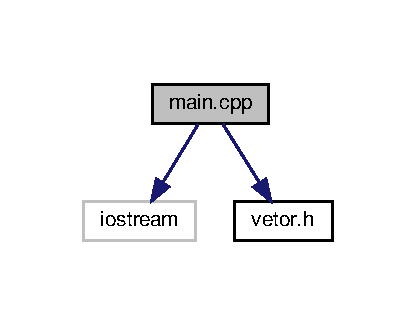
\includegraphics[width=200pt]{main_8cpp__incl}
\end{center}
\end{figure}
\subsection*{Functions}
\begin{DoxyCompactItemize}
\item 
int \hyperlink{main_8cpp_ae66f6b31b5ad750f1fe042a706a4e3d4}{main} ()
\end{DoxyCompactItemize}


\subsection{Function Documentation}
\mbox{\Hypertarget{main_8cpp_ae66f6b31b5ad750f1fe042a706a4e3d4}\label{main_8cpp_ae66f6b31b5ad750f1fe042a706a4e3d4}} 
\index{main.\+cpp@{main.\+cpp}!main@{main}}
\index{main@{main}!main.\+cpp@{main.\+cpp}}
\subsubsection{\texorpdfstring{main()}{main()}}
{\footnotesize\ttfamily int main (\begin{DoxyParamCaption}{ }\end{DoxyParamCaption})}


\hypertarget{vetor_8cpp}{}\section{vetor.\+cpp File Reference}
\label{vetor_8cpp}\index{vetor.\+cpp@{vetor.\+cpp}}
{\ttfamily \#include \char`\"{}vetor.\+h\char`\"{}}\newline
{\ttfamily \#include $<$cmath$>$}\newline
{\ttfamily \#include $<$iostream$>$}\newline
Include dependency graph for vetor.\+cpp\+:\nopagebreak
\begin{figure}[H]
\begin{center}
\leavevmode
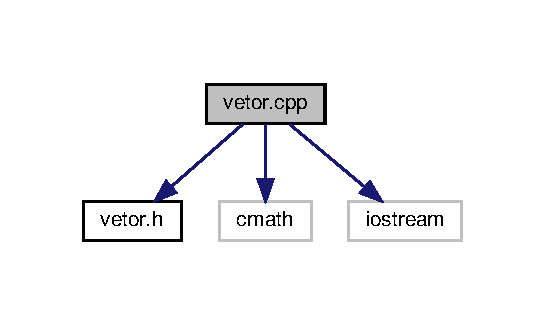
\includegraphics[width=262pt]{vetor_8cpp__incl}
\end{center}
\end{figure}
\subsection*{Functions}
\begin{DoxyCompactItemize}
\item 
\hyperlink{class_vetor}{Vetor} \hyperlink{vetor_8cpp_a94de46a0867046d0a49eb7e47b6d8e36}{operator$\ast$} (float a, \hyperlink{class_vetor}{Vetor} v)
\end{DoxyCompactItemize}


\subsection{Function Documentation}
\mbox{\Hypertarget{vetor_8cpp_a94de46a0867046d0a49eb7e47b6d8e36}\label{vetor_8cpp_a94de46a0867046d0a49eb7e47b6d8e36}} 
\index{vetor.\+cpp@{vetor.\+cpp}!operator$\ast$@{operator$\ast$}}
\index{operator$\ast$@{operator$\ast$}!vetor.\+cpp@{vetor.\+cpp}}
\subsubsection{\texorpdfstring{operator$\ast$()}{operator*()}}
{\footnotesize\ttfamily \hyperlink{class_vetor}{Vetor} operator$\ast$ (\begin{DoxyParamCaption}\item[{float}]{a,  }\item[{\hyperlink{class_vetor}{Vetor}}]{v }\end{DoxyParamCaption})}


\hypertarget{vetor_8h}{}\section{vetor.\+h File Reference}
\label{vetor_8h}\index{vetor.\+h@{vetor.\+h}}
This graph shows which files directly or indirectly include this file\+:\nopagebreak
\begin{figure}[H]
\begin{center}
\leavevmode
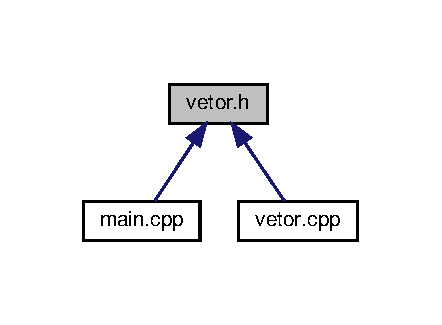
\includegraphics[width=212pt]{vetor_8h__dep__incl}
\end{center}
\end{figure}
\subsection*{Classes}
\begin{DoxyCompactItemize}
\item 
class \hyperlink{class_vetor}{Vetor}
\begin{DoxyCompactList}\small\item\em A classe \hyperlink{class_vetor}{Vetor} lida com vetores bidimensionais. \end{DoxyCompactList}\end{DoxyCompactItemize}
\subsection*{Functions}
\begin{DoxyCompactItemize}
\item 
\hyperlink{class_vetor}{Vetor} \hyperlink{vetor_8h_a94de46a0867046d0a49eb7e47b6d8e36}{operator$\ast$} (float a, \hyperlink{class_vetor}{Vetor} v)
\end{DoxyCompactItemize}


\subsection{Function Documentation}
\mbox{\Hypertarget{vetor_8h_a94de46a0867046d0a49eb7e47b6d8e36}\label{vetor_8h_a94de46a0867046d0a49eb7e47b6d8e36}} 
\index{vetor.\+h@{vetor.\+h}!operator$\ast$@{operator$\ast$}}
\index{operator$\ast$@{operator$\ast$}!vetor.\+h@{vetor.\+h}}
\subsubsection{\texorpdfstring{operator$\ast$()}{operator*()}}
{\footnotesize\ttfamily \hyperlink{class_vetor}{Vetor} operator$\ast$ (\begin{DoxyParamCaption}\item[{float}]{a,  }\item[{\hyperlink{class_vetor}{Vetor}}]{v }\end{DoxyParamCaption})}


%--- End generated contents ---

% Index
\backmatter
\newpage
\phantomsection
\clearemptydoublepage
\addcontentsline{toc}{chapter}{Index}
\printindex

\end{document}
